\documentclass[11pt,a4paper]{article}
\usepackage[margin=1in]{geometry}
\usepackage{hyperref}
\usepackage{enumitem}
\usepackage{graphicx}
\usepackage{xcolor}
\usepackage{tikz}
\usetikzlibrary{shapes.geometric, arrows.meta, positioning, calc, fit, backgrounds}

\tikzset{
  proc/.style={rectangle, rounded corners=2pt, draw=black!70, fill=blue!5,
               minimum height=7mm, text width=27mm, align=center, font=\scriptsize},
  term/.style={rectangle, rounded corners=8pt, draw=black!70, fill=black!8,
               minimum height=7mm, text width=25mm, align=center, font=\scriptsize},
  dec/.style={diamond, aspect=2.2, draw=black!70, fill=orange!12,
              inner sep=1pt, text width=21mm, align=center, font=\scriptsize},
  esc/.style={rectangle, rounded corners=2pt, draw=black!70, fill=red!8,
              minimum height=7mm, text width=25mm, align=center, font=\scriptsize},
  lay/.style={rectangle, rounded corners=2pt, draw=black!70, fill=blue!5,
              minimum height=7.5mm, text width=21mm, align=center, font=\scriptsize},
  mod/.style={rectangle, rounded corners=2pt, draw=black!70, fill=green!7,
              minimum height=6.5mm, text width=20mm, align=center, font=\scriptsize},
  grp/.style={rectangle, rounded corners=3pt, draw=black!45, dashed, inner sep=2.4mm},
  fl/.style={-{Latex[length=1.6mm]}, draw=black!70},
  lbl/.style={font=\scriptsize\itshape, inner sep=1.5pt},
  tier/.style={font=\scriptsize\bfseries, rotate=90, anchor=south, inner sep=1.5mm}
}

% -----------------------------------------------------
% bvraghav-tiet-ucs503p-article.sty
% -----------------------------------------------------

% Variable: Lab Instructor
\makeatletter \newcommand{\BvrSetLabInstructor}[1]{%
  \gdef\Bvr@LabInstructor{#1}}
% default
\newcommand{\Bvr@LabInstructor}{Ms. Anushka}
% public accessor
\newcommand{\BvrLabInstructorValue}{\Bvr@LabInstructor}
\makeatother

% Add subtitle
\usepackage{titling}
% -- Set title bold
\pretitle{\begin{center}\bfseries\fontsize{18bp}{18bp}\selectfont}
\makeatletter
\newcommand{\BvrSubtitle}[1]{%
  \posttitle{%
    \par\end{center}
    \begin{center}\large#1\end{center}
    \vskip 0.5em}%
}
\makeatother

% Hints in the section title(s)
\newcommand{\BvrHint}[1]{%
  {\normalfont\normalsize\itshape\hfill #1}}

% -----------------------------------------------------

\title{SHARP: A Smart Hostel Administration and Resource Platform}

\BvrSetLabInstructor{Ms. Anushka}

\BvrSubtitle{%
  Digital Workflows for Leave, Mess, Allotment, Maintenance and Laundry Services \\
  Project Proposal for UCS503  \\
  Submitted to: \BvrLabInstructorValue \\ \bfseries
  Thapar Institute of Engineering and Technology%
}

\author{
  Vaibhav Kansal, CSED, Roll No: \texttt{1024160097}
  \and
  Ali Ekram, CSED, Roll No: \texttt{1024160138}
  \and
  Riya Gupta, CSED, Roll No: \texttt{1024160122}
  \and
  Ayush Kamboj, CSED, Roll No: \texttt{1024160118}
}

\begin{document}
\maketitle

\section{Higher order goal}
This project aims to improve the accountability and traceability of everyday hostel
administration by replacing handwritten applications, physical registers and loosely tracked
complaints with a single auditable digital record. While the underlying goal is broader
institutional efficiency, the immediate engineering objective is to translate \emph{reliable,
traceable service delivery} across five hostel processes into a measurable, deployable
software solution.

\section{Time to value }
\begin{itemize}[leftmargin=0.7cm]
    \item We will deliver meaningful increments quickly by building authentication and role
    management first, then layering the five service modules on top so a usable core exists
    early.
    \item We will prioritize fast feedback by phasing delivery (leave,
    complaints, mess, allotment, laundry, then notifications and deployment) so a working
    minimum viable product exists even if later phases are unfinished.
    \item Success is defined by what can be delivered and measured in the first iteration
    (leave approval and complaint tracking), then improved based on warden and student
    feedback.
\end{itemize}

\section{Problem Statement}
Several routine hostel processes are partially manual or lack tracking. Five pain points
motivate the system:
\begin{itemize}[leftmargin=0.7cm]
    \item \textbf{Leave and passes:} handwritten applications and manual parent contact create
    paperwork and delay.
    \item \textbf{Mess feedback:} register-based collection discourages honesty because
    identity is visible to mess staff.
    \item \textbf{Allotment:} when cluster members pay at different times, a partly reserved
    room may be taken by others, breaking clusters.
    \item \textbf{Maintenance:} complaints stay unresolved for days, progress is untrackable
    and preferred repair slots go unhonoured.
    \item \textbf{Laundry:} lost or damaged items are reported informally if at all, so
    recurring problems (a particular day, batch or item type) go unnoticed.
\end{itemize}

\textbf{Why this matters now (contextual relevance):} With a hostel population large enough
that staff bandwidth is limited, even small tracking improvements (a unique complaint ID, an
expiry rule, a Service Level Agreement (SLA) timer) can noticeably reduce unresolved cases and disputes.

\section{Proposed Solution }
\subsection{Overview}
Build a \textbf{web-based} hostel administration platform with role-based workflows for
students, parents, wardens, caretakers, mess staff and laundry staff, comprising five modules:
\begin{itemize}[leftmargin=0.7cm]
    \item \textbf{Visitor and leave management:} day-out, regular and emergency requests
    routed as Student $\rightarrow$ Parent verification $\rightarrow$ Warden approval
    $\rightarrow$ digital pass with a unique ID.
    \item \textbf{Mess management:} categorised feedback on quality, hygiene, quantity, menu,
    timing and service, plus special meal requests; Feedback remains anonymous to mess staff, while internal records help prevent misuse
    \item \textbf{Allotment:} a temporary room reservation for a cluster leader that expires
    after a set window (e.g. 48 hours) if payment is incomplete, preserving clusters without
    weakening the fee requirement.
    \item \textbf{Complaint/maintenance management:} an ID and priority per report, caretaker
    assignment, and closure only after student verification, with Service Level Agreement (SLA) escalation to the
    warden.
    \item \textbf{Laundry issue tracking:} reports of missing, damaged, wrong or stained items,
    or delays, logged against each submission for later aggregation.
\end{itemize}

\subsection{Core workflow (complaint lifecycle example)}
\begin{enumerate}[leftmargin=0.7cm]
    \item Student files a complaint (category, preferred slot) and receives a complaint ID
    with an assigned priority.
    \item A caretaker is assigned and either agrees the proposed slot or offers an alternative;
    a Service Level Agreement (SLA) timer runs independently and notifies the warden if breached.
    \item The caretaker completes the repair and the student verifies resolution.
    \item If verified, the complaint closes; if not, it reopens against the same ID.
\end{enumerate}

\begin{figure}[!t]
\centering
\textit{The following figure illustrates the complete lifecycle of a maintenance complaint, from submission and caretaker assignment to resolution, verification, and closure.}
\vskip 0.5em
\resizebox{0.95\columnwidth}{!}{%
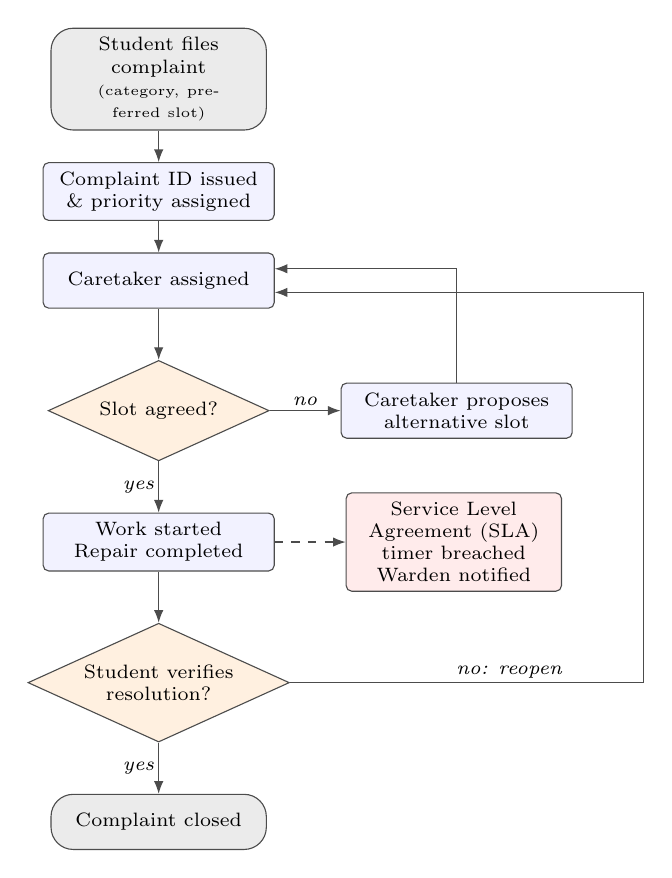
\begin{tikzpicture}[node distance=4mm]
\node[term] (a) {Student files complaint\\{\tiny(category, preferred slot)}};
\node[proc, below=of a] (b) {Complaint ID issued\\ \& priority assigned};
\node[proc, below=of b] (c) {Caretaker assigned};
\node[dec, below=6.5mm of c] (d) {Slot agreed?};
\node[proc, right=9mm of d] (e) {Caretaker proposes\\alternative slot};
\node[proc, below=6.5mm of d] (f) {Work started\\Repair completed};
\node[dec, below=6.5mm of f] (g) {Student verifies\\resolution?};
\node[term, below=6.5mm of g] (h) {Complaint closed};
\node[esc, right=9mm of f] (s) {Service Level Agreement (SLA) timer breached\\Warden notified};
\draw[fl] (a) -- (b);
\draw[fl] (b) -- (c);
\draw[fl] (c) -- (d);
\draw[fl] (d) -- node[lbl,above]{no} (e.west);
\coordinate (rr) at ($(e.east)+(9mm,0)$);
\draw[fl] (e.north) |- ($(c.east)+(0,1.5mm)$);
\draw[fl] (d) -- node[lbl,left]{yes} (f);
\draw[fl] (f) -- (g);
\draw[fl] (g) -- node[lbl,left]{yes} (h);
\draw[fl] (g.east) -- node[lbl,above,pos=0.62]{no: reopen} (g.east -| rr) |- ($(c.east)+(0,-1.5mm)$);
\draw[fl, dashed] (f.east) -- (s.west);
\end{tikzpicture}}
\caption{Figure 1: Maintenance Complaint Lifecycle.}
\label{fig:complaint}
\end{figure}

\subsection{Operational constraints for an educational, campus setting}
\begin{itemize}[leftmargin=0.7cm]
    \item Every sensitive endpoint checks both identity and permission, so a student cannot
    reach administrative dashboards, parent records or the identity behind anonymous feedback.
    \item Modules stay separable, so one module can change without redesigning the whole
    application.
    \item Design for deployability using common web hosting and managed databases.
\end{itemize}

\section{Solution Approach }
We focus on layered architecture, role-based access
control and workflow correctness rather than novel algorithm research.

\subsection{Layered architecture }
A layered architecture separates concerns across five tiers:
\begin{itemize}[leftmargin=0.7cm]
    \item \textbf{Interface:} role-specific portals for students/parents, wardens/admins, and
    caretaker/mess/laundry staff apps.
    \item \textbf{Application:} REST API endpoints, authentication (hashed credentials,
    tokens), and role-based access control.
    \item \textbf{Application Services:} the five modules (leave \& pass, mess feedback, allotment,
    complaints \& Service Level Agreement (SLA), laundry issues) plus notifications and analytics.
    \item \textbf{Data:} users, requests, complaints and reports; status history and audit
    records; backup and recovery.
    \item \textbf{External services (optional):} email, SMS or push notifications.
\end{itemize}

\subsection{CI/CD and fast delivery enabler}
CI/CD will be used to:
\begin{itemize}[leftmargin=0.7cm]
    \item Automatically build and run tests on every change.
    \item Produce repeatable deployment artifacts to staging.
    \item Enable safe and frequent releases of incremental features across the five modules.
\end{itemize}

\section{Evaluation Criterion }
We define success using measurable metrics tied to the core workflows.

\subsection{Primary evaluation metrics}
\begin{itemize}[leftmargin=0.7cm]
    \item \textbf{Complaint resolution time:} time between complaint filing and verified
    closure.
    \item \textbf{Service Level Agreement (SLA) compliance:} share of complaints closed within the defined SLA window.
    \item Attribution: measured from database timestamps (filing, assignment, completion,
    verification).
\end{itemize}

\subsection{Secondary evaluation metrics}
\begin{itemize}[leftmargin=0.7cm]
    \item \textbf{Paper Reduction:} Reduction in paper-based leave applications following the implementation of the system.
    \item \textbf{Leave approval time:} average time from student request to digital pass
    issuance.
    \item \textbf{Reopen count:} number of complaints reopened after a failed verification.
    \item \textbf{Laundry issues reported per month} and recurring-issue detection rate.
    \item \textbf{Reservation conflicts avoided:} clusters preserved through the expiry-based
    allotment mechanism.
\end{itemize}

\subsection{Pilot validation plan }
\begin{itemize}[leftmargin=0.7cm]
    \item Recruit a pilot hostel wing with student, warden, caretaker, mess and laundry staff
    roles.
    \item Compare metrics before/after within the iteration window by logging baseline
    estimates from existing manual records.
\end{itemize}

\section{Scalability }
The proposition should scale in both theoretical and practical senses.

\begin{enumerate}[leftmargin=0.7cm]
    \item \textbf{Scalable (theoretically):} The system should support growth in the number of
    students, requests and concurrent dashboard usage by:
    \begin{itemize}[leftmargin=0.7cm]
        \item decoupling the interface, application and business-logic layers,
        \item keeping modules separable so one can change without redesigning the rest,
        \item designing the schema to admit further hostels without redesign.
    \end{itemize}

    \item \textbf{Operationally deployable (practically):} The system should run on common web
    hosting:
    \begin{itemize}[leftmargin=0.7cm]
        \item a managed database with backup and recovery,
        \item token-based authentication and role-based access control,
        \item a CI/CD pipeline for staging/production deployment.
    \end{itemize}
\end{enumerate}

\section{Engine availability heuristic}
A mature set of ``engines'' (tooling/services) is available to implement this as a web-based
project. The layers are specified by responsibility, not by product, so the implementation
stack will be finalised at build time once hosting, library maturity and team familiarity are
weighed:
\begin{itemize}[leftmargin=0.7cm]
    \item Web framework for REST APIs and role-specific reactive pages (e.g. React with
    Tailwind CSS).
    \item Managed backend runtime and database (e.g. Node.js with Express and MongoDB).
    \item Token-based authentication with hashed credentials.
    \item Test framework for unit/integration tests.
    \item CI runner and staging deployment target.
    \item Optional notification services (email, SMS, push).
\end{itemize}
No workflow rule, role definition or metric depends on a particular language, so deferring the
final stack choice costs nothing.

\section{Project scope and deliverables }
\subsection{Initial deliverable }
\begin{itemize}[leftmargin=0.7cm]
    \item Authentication and role-based access control for all six roles
    \item Leave and visitor pass workflow: Student, Parent, and Warden
    \item Complaint lifecycle: filing, assignment, SLA timer, verified closure
    \item Basic logging and timestamps for resolution-time measurement
    \item CI: build + backend unit tests + linting
    \item CD to staging with a single command or pipeline job
\end{itemize}

\subsection{Subsequent deliverables}
\begin{itemize}[leftmargin=0.7cm]
    \item Mess feedback module with anonymity and abuse-deterrence records
    \item Allotment module with temporary reservation and expiry
    \item Laundry issue tracking with aggregated recurring-issue reports
    \item Notification layer (email/SMS optional; can start in-app)
    \item Admin/warden analytics dashboard
\end{itemize}

\section{Risk Management}
\begin{itemize}[leftmargin=0.7cm]
    \item \textbf{Unauthorised access:} mitigated by role-based authentication.
    \item \textbf{Forged parent approval:} mitigated by secure tokens plus warden
    verification.
    \item \textbf{Abuse of anonymous mess feedback:} mitigated by rate limits and internal
    audit records.
    \item \textbf{Premature loss of a room reservation:} mitigated by expiry rules and
    transactional validation.
    \item \textbf{Disputed laundry loss:} mitigated by timestamped reports tied to each
    submission.
\end{itemize}

\section{Summary}
This project proposes SHARP, a web-based hostel administration platform that brings five hostel processes—leave and passes, mess feedback, room allotment, maintenance complaints, and laundry—into one system. The project will implement role-based access, digital workflows, complaint tracking, verification, notifications, and basic logging. The initial implementation will focus on authentication, leave and visitor pass management, and the maintenance complaint lifecycle, followed by the remaining modules. The aim is to make hostel processes easier to manage, track, and verify through a single digital platform.

\end{document}